% Build:  xelatex report.tex   (twice, for cross-references)
%
% hyperref is loaded directly rather than via the bookmark package. TeX Live
% 2026 ships bookmark v1.32 against hyperref v7.01p, and in that pairing
% bookmark never loads its xetex driver, so \bookmark stays undefined and the
% build fails at the first \section.

\documentclass[11pt,a4paper]{article}

\usepackage{fontspec}
\usepackage[a4paper,margin=2.4cm]{geometry}
\usepackage{amssymb}
\usepackage{booktabs}
\usepackage{array}
\usepackage{fancyvrb}
\usepackage{enumitem}
\usepackage{xcolor}
\usepackage{titlesec}
\usepackage{microtype}
\usepackage{tikz}
\usetikzlibrary{arrows.meta,positioning,fit}
\usepackage{hyperref}

\definecolor{Accent}{HTML}{1F3D7A}
\definecolor{RuleGrey}{HTML}{C8CDD4}

\hypersetup{
  colorlinks=true, linkcolor=black, urlcolor=Accent,
  pdftitle={Multimodal RAG for the Sri Lanka Tourism Sector},
  pdfsubject={SCS 4203 Database III, Assignment 2}
}

\setlength{\parskip}{0.5em}
\setlength{\parindent}{0pt}
\renewcommand{\arraystretch}{1.15}

\titleformat{\section}{\large\bfseries\color{Accent}}{\thesection}{0.6em}{}
\titlespacing*{\section}{0pt}{1.3em}{0.4em}
\titleformat{\subsection}{\normalsize\bfseries}{\thesubsection}{0.5em}{}
\titlespacing*{\subsection}{0pt}{0.9em}{0.3em}

\setlist[itemize]{leftmargin=1.3em,topsep=0.2em,itemsep=0.2em}
\setlist[enumerate]{leftmargin=1.5em,topsep=0.2em,itemsep=0.2em}

\DefineVerbatimEnvironment{codeblock}{Verbatim}
  {fontsize=\scriptsize,frame=single,rulecolor=\color{RuleGrey},
   framesep=6pt,baselinestretch=0.98}

\newcommand{\code}[1]{\texttt{\small #1}}

\tikzset{
  blk/.style   = {draw=RuleGrey, rounded corners=2pt, align=center,
                  font=\footnotesize, inner sep=4pt, minimum height=9mm},
  wide/.style  = {blk, fill=black!3, text width=88mm},
  store/.style = {blk, fill=Accent!6, text width=31mm, minimum height=15mm},
  flow/.style  = {-{Stealth[length=4pt,width=3pt]}, draw=black!50, line width=0.4pt},
  tag/.style   = {font=\scriptsize\bfseries\color{Accent}, anchor=east},
}

\begin{document}

\begin{center}
  {\Large\bfseries Multimodal Retrieval-Augmented Generation\\[0.15em]
   for the Sri Lanka Tourism Sector\par}
  \vspace{0.7em}
  {\normalsize SCS 4203, Database III, Assignment 2\par}
  \vspace{1em}
  \begin{tabular}{@{}ll@{}}
    \toprule
    Student 1 & \textit{[Name]}, \textit{[Index No]} \\
    Student 2 & \textit{[Name]}, \textit{[Index No]} \\
    Date      & \textit{[Submission date]} \\
    \bottomrule
  \end{tabular}
\end{center}

\vspace{0.8em}

% ---------------------------------------------------------------------------
\section{System architecture}

A question like "which waterfalls are over 100 metres tall" filters on a
number. "Where can I see colonial-era fortifications beside the sea" names no
column, so it has to be matched on meaning. A photograph is neither. Each kind
needs a different store: a relational database answers exactly but cannot
match on meaning, a text-embedding index matches on meaning but cannot filter
reliably, and an image-embedding index handles visual similarity that neither
of the others can express. This system routes each question to whichever
stores can answer it, then merges the results before the language model sees
them.

\begin{center}
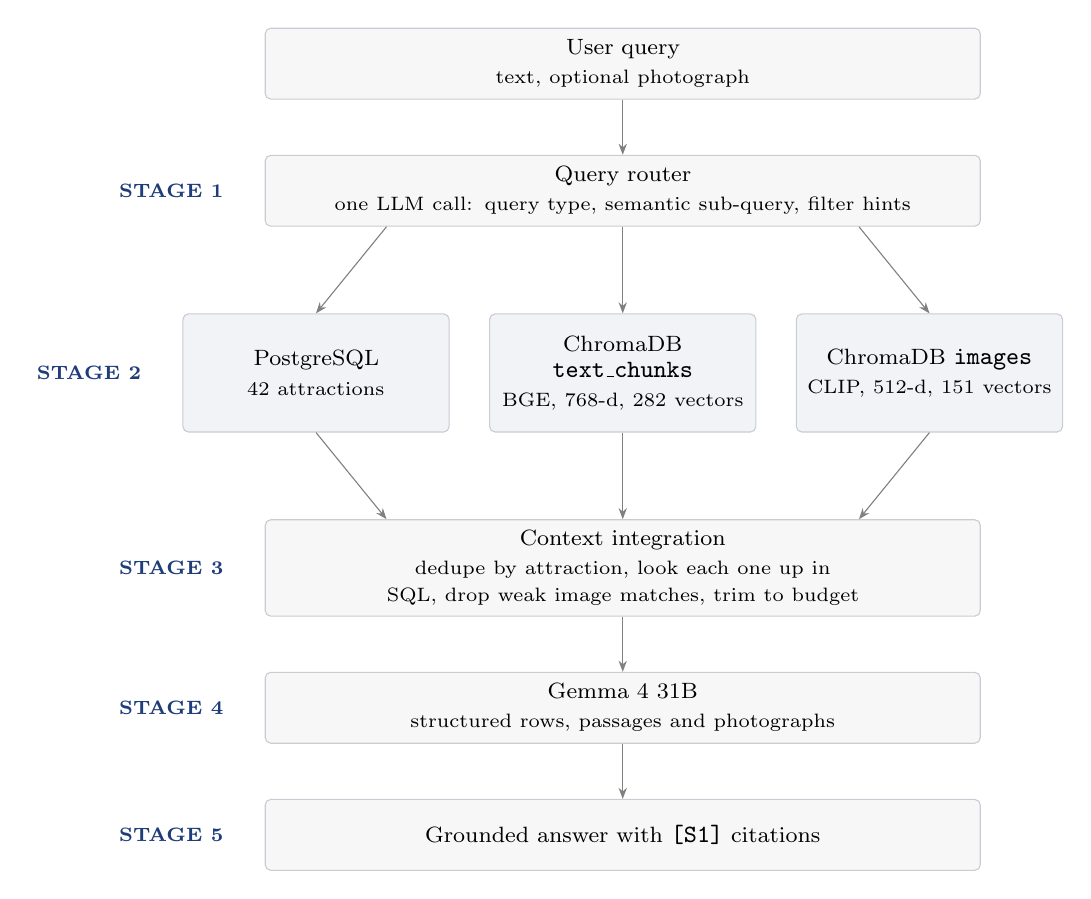
\begin{tikzpicture}[node distance=7mm]

  \node[wide] (query) {User query\\[1pt]\scriptsize text, optional photograph};

  \node[wide, below=of query] (router)
    {Query router\\[1pt]\scriptsize one LLM call: query type, semantic sub-query, filter hints};

  \node[store, below=11mm of router] (text)
    {ChromaDB \code{text\_chunks}\\[1pt]\scriptsize BGE, 768-d, 282 vectors};
  \node[store, left=5mm of text] (sql)
    {PostgreSQL\\[1pt]\scriptsize 42 attractions};
  \node[store, right=5mm of text] (img)
    {ChromaDB \code{images}\\[1pt]\scriptsize CLIP, 512-d, 151 vectors};

  \node[wide, below=11mm of text] (integrate)
    {Context integration\\[1pt]\scriptsize dedupe by attraction, look each one up in SQL,
     drop weak image matches, trim to budget};

  \node[wide, below=of integrate] (llm)
    {Gemma 4 31B\\[1pt]\scriptsize structured rows, passages and photographs};

  \node[wide, below=of llm] (answer)
    {Grounded answer with \code{[S1]} citations};

  \draw[flow] (query) -- (router);

  \draw[flow] ([xshift=-30mm]router.south) -- (sql.north);
  \draw[flow] (router.south)               -- (text.north);
  \draw[flow] ([xshift=30mm]router.south)  -- (img.north);

  \draw[flow] (sql.south)  -- ([xshift=-30mm]integrate.north);
  \draw[flow] (text.south) -- (integrate.north);
  \draw[flow] (img.south)  -- ([xshift=30mm]integrate.north);

  \draw[flow] (integrate) -- (llm);
  \draw[flow] (llm) -- (answer);

  \node[tag] at ([xshift=-4mm]router.west)    {STAGE 1};
  \node[tag] at ([xshift=-4mm]sql.west)       {STAGE 2};
  \node[tag] at ([xshift=-4mm]integrate.west) {STAGE 3};
  \node[tag] at ([xshift=-4mm]llm.west)       {STAGE 4};
  \node[tag] at ([xshift=-4mm]answer.west)    {STAGE 5};

\end{tikzpicture}
\end{center}

Stage 3, described in Section \ref{sec:integrate}, is what makes this a
combined system rather than three independent search boxes. Section
\ref{sec:eval} measures whether combining them actually helps.

% ---------------------------------------------------------------------------
\section{Database design}

The knowledge base covers three categories, waterfalls, beaches, and
historical sites and temples, chosen from the brief's list because each
exercises a different part of the schema: waterfalls carry numeric attributes,
heritage sites carry categorical and boolean ones, and beaches are described
mostly in prose. It holds 42 attractions across 19 districts, 14 per category,
with 282 text chunks and 164 photographs.

\begin{center}
\begin{tabular}{@{}lr@{}}
\toprule
\textbf{Asset} & \textbf{Count} \\
\midrule
Text chunks from Wikipedia          & 205 \\
Text chunks from AmazingLanka       & 77 \\
Photographs indexed                 & 151 \\
Photographs held out for evaluation & 13 \\
\bottomrule
\end{tabular}
\end{center}

Wikipedia alone covers the three categories unevenly: the Sigiriya article runs
to 2{,}660 words, while Bambarakanda Falls, the tallest waterfall in Sri Lanka,
is a 131-word stub. AmazingLanka, a Sri Lankan travel encyclopaedia read
through its public REST API, fills in exactly the attractions Wikipedia treats
thinly, and supplied text for 26 of the 42 attractions. Trekking difficulty is
not reliably available from either source and was entered by hand in
\code{data/seeds/attractions.csv}. Entrance fees, swimming safety, surf season
and accessibility notes were planned as columns too, but neither source gave
a usable value for any of the 42 attractions, so they were dropped from the
schema rather than kept as columns that were always empty.

\subsection{Relational schema}

\begin{codeblock}
attractions (
    id SERIAL PRIMARY KEY,
    name TEXT NOT NULL UNIQUE,
    category TEXT NOT NULL CHECK (category IN ('waterfall','beach','heritage')),
    district TEXT, province TEXT, latitude FLOAT8, longitude FLOAT8,
    height_m NUMERIC(6,1),        -- waterfalls
    trekking_difficulty TEXT,     -- waterfalls
    era TEXT,                     -- heritage
    unesco_status BOOLEAN,        -- heritage
    dress_code TEXT,              -- heritage
    best_season TEXT, summary TEXT, wiki_url TEXT
)

images (
    id SERIAL PRIMARY KEY,
    attraction_id INT NOT NULL REFERENCES attractions(id) ON DELETE CASCADE,
    file_path TEXT NOT NULL, caption TEXT,
    source_url TEXT, license TEXT, is_held_out BOOLEAN DEFAULT FALSE
)

documents (
    id SERIAL PRIMARY KEY,
    attraction_id INT NOT NULL REFERENCES attractions(id) ON DELETE CASCADE,
    chunk_index INT NOT NULL, chunk_text TEXT NOT NULL,
    source TEXT CHECK (source IN ('wikipedia','amazinglanka')), source_url TEXT,
    UNIQUE (attraction_id, chunk_index)
)
\end{codeblock}

Indexed on \code{category}, \code{district} and \code{height\_m}, plus
\code{attraction\_id} on both child tables. Every image row records its
source and licence, so provenance stays traceable back to Commons.

\subsection{Design decisions}

\textit{One wide table instead of per-category subtypes.} The normalised
design would put \code{height\_m} in a \code{waterfalls} table and
\code{dress\_code} in a \code{heritage\_sites} table, both joined to a common
supertype. That is cleaner, since it makes it structurally impossible to set a
waterfall's height on a beach. We rejected it because the SQL retriever is a
language model writing queries from a schema in its prompt
(Section \ref{sec:sqlretrieval}): every extra table is another join it has to
get right, and a single table keeps the generated SQL a plain
\code{SELECT}. The cost is that most category-specific columns are NULL on any
given row, 28 of 42 rows have no \code{height\_m}, correctly, since only the 14
waterfalls have a height. This is the decision we would most want to revisit.

\textit{\code{unesco\_status} marks inscribed sites only.} Six attractions are
UNESCO World Heritage Sites. Ruwanwelisaya, Jetavanaramaya and Isurumuniya
stand inside the Sacred City of Anuradhapura, itself one inscribed site, so
flagging them separately would make "how many UNESCO sites are there" answer
nine and count one site four times.

\textit{\code{documents} holds the authoritative text.} ChromaDB stores only
vectors, ids and filter metadata, so the whole vector index can be rebuilt
from PostgreSQL by re-running \code{embed.py}.

\subsection{Vector store}

\begin{center}
\small
\begin{tabular}{@{}llrr@{}}
\toprule
\textbf{Collection} & \textbf{Encoder} & \textbf{Dim} & \textbf{Vectors} \\
\midrule
\code{text\_chunks} & \code{BAAI/bge-base-en-v1.5} & 768 & 282 \\
\code{images}       & \code{clip-ViT-B-16}         & 512 & 151 \\
\bottomrule
\end{tabular}
\end{center}

Both use cosine distance. \code{text\_chunks} carries \code{attraction\_id},
\code{name}, \code{category}, \code{district} and the source fields as
metadata; \code{images} carries the same minus the source fields, plus
\code{file\_path}. The two collections stay separate because the encoders
produce vectors in unrelated spaces: comparing a BGE vector to a CLIP vector
raises no error, it just returns meaningless neighbours.

% ---------------------------------------------------------------------------
\section{Embedding generation}

Both encoders run locally, so ingestion and indexing need no API access. Only
routing, SQL generation and answering call an external model.

\subsection{Text}

Articles are split into overlapping windows of 220 words with 50 words of
overlap, and each chunk is prefixed with its attraction's name before
encoding. Without it, a chunk reading "It is 263\,m high and has a single
drop" tells neither the embedding nor the model which attraction "it" is.
Wikipedia's trailing sections and AmazingLanka's navigation blocks and
star-rating widget are stripped first. Vectors are L2-normalised, so cosine
distance matches the dot product.

\subsection{Images}

Photographs are converted to RGB, resized so the longest edge is 512\,px, and
encoded with CLIP ViT-B/16 into 512 dimensions. CLIP was chosen because it
puts images and text in one shared space, which gives two capabilities from
one index: image-to-image search when a photograph is uploaded, and
text-to-image search when someone types a description instead. Thirteen
photographs, the fourth of every waterfall, are held out of the index to
serve as an evaluation set of images the system has not seen.

\subsection{Choosing the encoders}

Both encoders were selected by measurement. Text encoders were scored on the
22 semantic and hybrid evaluation questions, image encoders on the 13
held-out photographs.

\begin{center}
\small
\begin{tabular}{@{}lrrrr@{}}
\toprule
\textbf{Text encoder} & \textbf{dim} & \textbf{R@1} & \textbf{R@3} & \textbf{MRR} \\
\midrule
\code{bge-base-en-v1.5}          & 768 & 68.2\% & \textbf{90.9\%} & \textbf{0.792} \\
\code{bge-small-en-v1.5}         & 384 & 68.2\% & 81.8\% & 0.761 \\
\code{nomic-embed-text-v1.5}     & 768 & 63.6\% & 86.4\% & 0.746 \\
\code{bge-small-en-v1.5} + query prefix & 384 & 63.6\% & 77.3\% & 0.739 \\
\code{e5-base-v2}                & 768 & 59.1\% & 77.3\% & 0.689 \\
\bottomrule
\end{tabular}
\end{center}

\begin{center}
\small
\begin{tabular}{@{}lrrrr@{}}
\toprule
\textbf{Image encoder} & \textbf{dim} & \textbf{top-1} & \textbf{top-3} & \textbf{MRR} \\
\midrule
\code{clip-ViT-B-16} & 512 & \textbf{61.5\%} & \textbf{69.2\%} & \textbf{0.673} \\
\code{clip-ViT-L-14} & 768 & 61.5\% & 61.5\% & 0.646 \\
\code{clip-ViT-B-32} & 512 & 30.8\% & 69.2\% & 0.487 \\
\bottomrule
\end{tabular}
\end{center}

BGE ships with an optional instruction prefix for queries, and adding it made
retrieval worse here, so it is not used. Nomic-embed-text's 8192-token context
is never exercised by 220-word chunks, and it scored below the smaller BGE
model while also requiring \code{trust\_remote\_code}. On images, moving from
32-pixel to 16-pixel patches doubled top-1 accuracy, and the larger ViT-L/14
did not help further. The text comparison turns on two questions out of 22 and
the image comparison on four photographs out of 13, so these results point in
a direction rather than settle it definitively.

% ---------------------------------------------------------------------------
\section{Retrieval workflow}
\label{sec:retrieval}

\subsection{Routing}

One LLM call classifies the question as \code{structured}, \code{semantic},
\code{image} or \code{hybrid} and extracts a semantic sub-query plus any
category or district the question restricts itself to. The class decides
which retrievers run.

\begin{center}
\begin{tabular}{@{}lccc@{}}
\toprule
\textbf{Query type} & \textbf{SQL} & \textbf{Text} & \textbf{Images} \\
\midrule
\code{structured} & \checkmark &            &            \\
\code{semantic}   &            & \checkmark &            \\
\code{image}      &            &            & \checkmark \\
\code{hybrid}     & \checkmark & \checkmark & \checkmark \\
\bottomrule
\end{tabular}
\end{center}

An uploaded photograph always forces image retrieval. If the routing call
fails after its retries the query falls back to \code{hybrid} and runs
everything, which is slower but never retrieves less than the question needs.

\subsection{Structured retrieval}
\label{sec:sqlretrieval}

The model is given the schema and writes a \code{SELECT}, which is checked
before it runs: anything that does not start with \code{SELECT}, contains a
second statement, or matches \code{INSERT}, \code{UPDATE}, \code{DELETE},
\code{DROP}, \code{ALTER}, \code{TRUNCATE}, \code{GRANT}, \code{REVOKE},
\code{CREATE} or \code{COPY} is rejected. The prompt also lists the distinct
values of every low-cardinality column, since a model given only the schema
will write valid-looking predicates such as \code{province = 'Central
Province'} against a column that actually stores \code{'Central'}, which
returns nothing and looks identical to the attraction not existing.

\subsection{Vector retrieval}

Semantic search embeds the sub-query and takes the top $k$ chunks. If the
router identified a category or district, that becomes a ChromaDB metadata
filter applied before the vector comparison, so a question about temples near
Kandy searches only Kandy instead of hoping the embedding encodes the
district. A filter that matches nothing falls back to an unfiltered search.
Image search embeds either the uploaded photograph or the text sub-query
against the same CLIP collection.

\subsection{Context integration}
\label{sec:integrate}

This is where the relational and vector stores meet. Candidates are ranked by
attraction rather than by chunk, since vector search often returns several
chunks and photographs belonging to the same place. Every attraction found by
either vector store is then looked up in PostgreSQL and its full row added to
the context, so a purely semantic match still arrives carrying its exact
district, era, UNESCO status and coordinates. Weak image matches are dropped
using the gap below the best score rather than a fixed threshold, since CLIP
similarities sit in a narrow band regardless of relevance.

\subsection{Generation}

The context goes to Gemma 4 31B along with the retrieved photographs as image
parts rather than filenames, so the generation is genuinely multimodal. The
system prompt tells the model to answer only from the context, cite passages
as \code{[S1]}, and reply that the knowledge base does not cover the question
rather than filling the gap from general knowledge.

% ---------------------------------------------------------------------------
\section{Evaluation}
\label{sec:eval}

\subsection{Method}

We wrote 36 evaluation questions, each labelled with its expected query type
and the attractions a correct answer has to be grounded in: 8 structured, 16
semantic, 6 hybrid and 6 image. Four things were measured: router accuracy
over all 36, text retrieval over the 22 semantic and hybrid questions
(Recall@$k$ and MRR, ranked by attraction), image retrieval on the 13
held-out photographs, and an ablation comparing SQL-only, semantic-only and
the full hybrid pipeline by \textit{context recall}, how often the expected
attraction reaches the model. Context recall was chosen over judging answer
wording because it is objective: if the right attraction never reaches the
model, no prompt can fix the answer.

\subsection{Results}

\begin{center}
\begin{tabular}{@{}lr@{}}
\toprule
\textbf{Metric} & \textbf{Result} \\
\midrule
Router accuracy   & 86.1\% (31/36) \\
Text Recall@1     & 68.2\% \\
Text Recall@3     & 90.9\% \\
Text Recall@5     & 95.5\% \\
Text MRR          & 0.792 \\
Image top-1       & 61.5\% (n=13) \\
Image top-3       & 69.2\% (n=13) \\
\midrule
Context recall, SQL only      & 52.9\% \\
Context recall, semantic only & 91.7\% \\
Context recall, hybrid        & \textbf{97.2\%} \\
\bottomrule
\end{tabular}
\end{center}

\subsection{Discussion}

The ablation is clearest broken down by question type.

\begin{center}
\small
\begin{tabular}{@{}lrrrr@{}}
\toprule
\textbf{Question type} & \textbf{n} & \textbf{SQL only} & \textbf{Semantic only} & \textbf{Hybrid} \\
\midrule
structured & 8  & 88\%  & 75\%   & \textbf{100\%} \\
semantic   & 16 & 36\%  & 94\%   & 94\% \\
image      & 6  & 0\%   & 100\%  & 100\% \\
hybrid     & 6  & 100\% & 100\%  & 100\% \\
\midrule
all        & 36 & 52.9\% & 91.7\% & \textbf{97.2\%} \\
\bottomrule
\end{tabular}
\end{center}

The relational store alone fails in a structured way: it cannot answer
questions with no matching column, such as one about frescoes or one asking
what a photograph shows. Combining the stores beats either alone, most
clearly on structured questions, where hybrid retrieval reaches every
attraction that SQL and semantic search individually miss.

The "image" row is worth a caveat. These questions are still typed text
("show me photographs of a tall narrow waterfall"), so a description like
"an ancient rock fortress" already matches the attraction's text chunks
without the image index doing any work, which is why semantic-only also
reaches 100\% there. This table cannot show what the image index is actually
for: answering with an uploaded photograph, which no text query can express.
That capability is measured separately in the image retrieval results above.

\textbf{Routing.} 86.1\% (31/36) is the weakest figure, and the five errors
split into two kinds. Three are over-classification to \code{hybrid}, two
semantic questions and one structured question, which costs time and context
budget but not correctness, since \code{hybrid} retrieves a superset. Two are
narrower: hybrid questions routed as structured instead. That is the more
consequential kind, since a narrower strategy can lose information, though in
this set it did not, because every hybrid-labelled question is also fully
answerable from the relational store alone (the hybrid row above reads 100\%
under SQL only). Image questions were classified perfectly. The router prompt
was not tuned against these questions, since the evaluation set is the only
measurement available and tuning against it would leave nothing left to
evaluate on.

\textbf{Text retrieval.} Recall@3 of 90.9\% and MRR of 0.792 mean the
right attraction is usually at or near the top of the ranking. Recall@1 of
68.2\% is the figure with the most room left, and reranking the retrieved
chunks is the obvious way to raise it.

\textbf{Image retrieval.} Top-1 of 61.5\% (n=13) is measured on the hardest
available task, since all 13 held-out photographs are waterfalls and the
encoder has to tell visually similar falls apart rather than tell a beach
from a temple. Top-3 of 69.2\% (n=13) matters more in practice, since the
shortlist is what reaches the model.

\subsection{Limitations}

\begin{itemize}
  \item Entrance fees, swimming safety, surf season and accessibility are not
        tracked at all: neither source gave a usable value for any
        attraction, so these were dropped from the schema rather than kept
        as columns that were always NULL. A question about any of them falls
        through to semantic search, which does not have the information
        either, and the system says so rather than guessing.
  \item There is no reranking of retrieved chunks, which is the most direct
        way to raise Recall@1.
  \item Semantic search has no per-attraction diversity cap: one query
        returned six chunks all belonging to the same place.
  \item The \code{SELECT}-only guard is enforced in application code rather
        than at the database level, and the database user is not read-only.
  \item Thirty-six questions and thirteen held-out images are still a small
        sample; the gap between semantic-only and hybrid context recall
        rests on 2 of 36 questions.
  \item National parks and wildlife were dropped for time. Distinct species
        are easier to tell apart visually than one waterfall from another,
        so their absence makes the image retrieval task harder than it would
        otherwise be.
\end{itemize}

% ---------------------------------------------------------------------------
\section{Implementation}

\begin{center}
\begin{tabular}{@{}ll@{}}
\toprule
Language         & Python 3.12 \\
Relational store & PostgreSQL 16 (Docker) \\
Vector store     & ChromaDB (persistent, local) \\
Encoders         & \code{bge-base-en-v1.5}, \code{clip-ViT-B-16} \\
Generation       & Gemma 4 31B (\code{gemma-4-31b-it}) \\
Interface        & Streamlit \\
\bottomrule
\end{tabular}
\end{center}

\begin{codeblock}
src/config.py     tunable parameters
src/schema.sql    relational schema
src/sources.py    Wikipedia / AmazingLanka / Commons clients
src/ingest.py     web sources -> PostgreSQL
src/embed.py      PostgreSQL -> ChromaDB
src/retrieval.py  router and the three retrievers
src/generate.py   LLM prompting and answering
src/pipeline.py   the five stages
src/evaluate.py   evaluation harness
app.py            Streamlit interface
\end{codeblock}

The interface shows the routing decision, the SQL that ran, the retrieved
chunks with their similarity scores, the matched photographs and the exact
context sent to the model, so an answer can always be traced back to what
produced it.

Ingest is destructive and reproducible: each run re-applies the schema and
rebuilds from the curated CSV plus the web sources, committing per attraction
so a network failure does not lose earlier work. Installation and run
instructions are in \code{README.md}.

% ---------------------------------------------------------------------------
\section*{Acknowledgements}

\begin{itemize}
  \item Wikipedia and Wikimedia Commons, for descriptive text, coordinates
        and all 164 photographs, under CC BY-SA. Per-image licence and
        author are stored in the \code{images} table.
  \item AmazingLanka (\url{https://amazinglanka.com/wp/}), for additional
        text on 26 attractions, used for non-commercial academic purposes
        with attribution. No images were taken from this source.
  \item Models: \code{BAAI/bge-base-en-v1.5} (MIT), OpenAI CLIP via
        \code{sentence-transformers}, Google Gemma via the Gemini API.
  \item Libraries: PostgreSQL, ChromaDB, sentence-transformers, PyTorch,
        Streamlit, psycopg, Pillow, requests, google-genai.
\end{itemize}

AI-assisted development tools were used during implementation. The design
decisions, evaluation method and analysis are our own.

\end{document}
